\newpage
\section{Google API Service Implementation}
    Following the design in the section \ref{ssec:srp} the class 
    GoogleAPIService is responsible to make the request to the Google
    Direction API and return the result to the presenter which will be
    processed by the I/O service. The fig \ref{fig:directionServiceSeqDiagram}
    describes the object interactions and the messages exchanged during the
    single request that is made to receive a navigation data as described in
    the list \ref{code: googleAPi Result}.
    \par
        As described earlier to make http request a HTTP client is required and Retrofit
        is being used. Some parameters like the base endpoint of googleAPI (where the http
        request would be made. i.e. https://maps.googleapis.com/ ), connection, read timeouts
        to ensure the request is terminated 
        in case of situation when the server is not available 
        and error handling methods are configured in 
        GoogleDirectionMiddleWare. Please see the appendix 
        \ref{code:retrofitConfig} to check the configuration.        

    \begin{figure}[htbp!]
        \centering 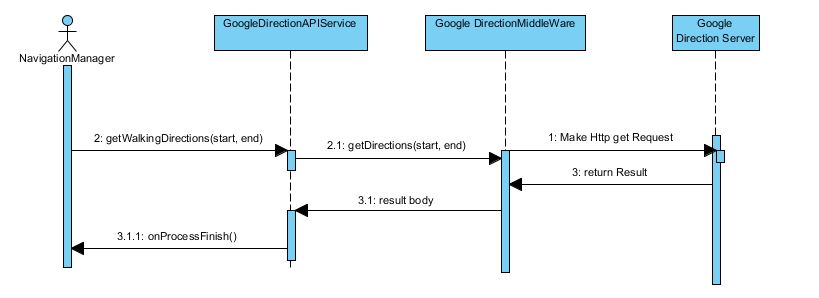
\includegraphics[scale=0.75]{grafiken/seqDigGoogleAPI.jpg}
        \caption{Sequence Diagram: Describing the functonality of the Google API service}
        \label{fig:directionServiceSeqDiagram}
    \end{figure}